% !TeX root = ../main.tex
% Add the above to each chapter to make compiling the PDF easier in some editors.

\chapter{Datasets}\label{chapter:datasets}
This thesis shows the performance of different active learning algorithms, pre-training methods and training strategies on three biomedical image datasets, as shown in Figure \ref{fig:datasets_composition}.

\begin{figure}[htbp]
\centering
\captionsetup{format=plain}
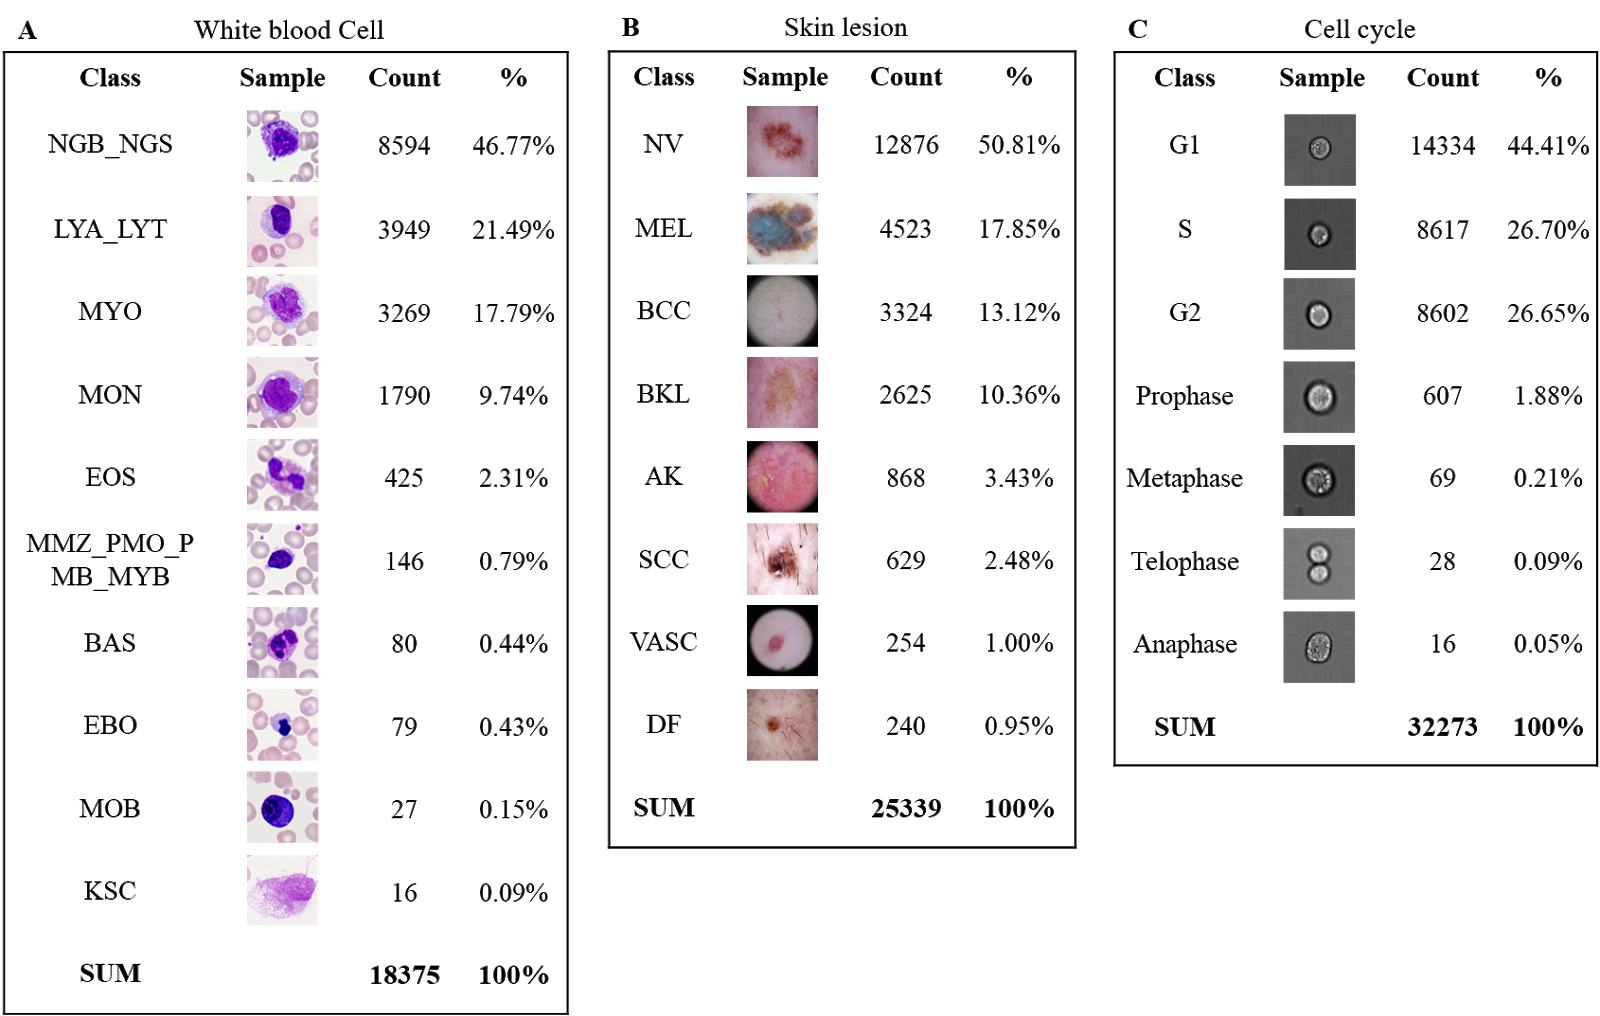
\includegraphics[width=0.95\textwidth]{figures/fig_datasets_composition.png}
\caption{The biomedical image datasets shown in this thesis have high class imbalance, low levels of contrast between different colors and a high level of similarity between different classes (A) White blood cell: This dataset contains 18357 (128x128) single-cell images. They are taken from peripheral blood smears of 100 patients diagnosed with AML, as well as 100 patients without any symptoms of the disease. \cite{matek2019, clark2013}. (B) Skin lesion: This dataset contains 25339 (128x128) images obtained using Dermoscopy. The images are classified into eight classes which specify different skin cancer types. \cite{codella2018, combalia2019, tschandl2018}. (C) Cell cycle: A dataset comprising 32272 images (64x64 pixel) of Jurkat cells in seven different cell cycle stages created by imaging flow cytometry \cite{eulenberg2017}.}
\label{fig:datasets_composition}
\end{figure}

\newpage

% rework these sections to make them different from what it says on their websites
\section{White Blood Cells}

The White Blood Cells Dataset contains 18357 single-cell images labeled by experts taken from peripheral blood smears of 100 patients diagnosed with AML, as well as 100 patients without any symptoms of the disease. 

White blood cells, also known as leukocytes or leucocytes, are the cells which protect the body from foreign objects and infections. White blood cells are found throughout the body including the blood.

AML is a cancer occurring in the myeloid line of blood cells. Its symptoms include the rapid growth of abnormal cells which interfere with normal blood cells production due to a build-up in the bone marrow and the blood. Symptoms can include continuous feeling of tiredness, being out of breath frequently, and high risk of infection. At certain occasions, the cancer can metastasize and spread to other organs of the body. AML progresses quickly and can prove to be fatal in a matter of months. AML is initially treated using chemotherapy. The goal of chemotherapy is to set a remission in motion. Other treatments include radiation therapy or a stem cell transplant. The treatment is guided by the type of mutation present within the body. This also dictates, how long a person is likely to live.

During the formulation of the dataset, the malignant and non-malignant white blood cells were classified into a standard morphological classification scheme. To quantify account of uncertainties between the expert labeling, a subset of images was re-annotated up to two times.

The dataset has been used as the primary dataset for testing different active learning algorithms, training strategies and pre-training methods.

\section{Skin Lesion}

The Skin Lesion dataset is developed by The International Skin Imaging Collaboration (ISIC): Melanoma project. The goal of the melanoma project is the application of medical imaging using computational technologies for detection of melanoma and eventually the reduction of melanoma mortality.

Melanoma, also called malignant melanoma, is a type of skin cancer. It is developed within the melanocytes cells. Melanocytes are responsible for producing pigments in the skin. Melanomas can also occur in other organs such as the mouth, intestines and the eye. About 25\% of melanomas develop from moles. Symptoms such as increase in the size of a mole, irregular edges, color changes, itchiness or skin breakdown can indicate melanoma.

Melanoma treatment heavily depends on early detection. If detected in its early stages, Melanoma is readily curable. Skin lesion imaging can not only help with the education of experts and the public but it can also be used for automated diagnosis, decision support in clinics and teledermatology. The quality of skin lesion imaging is hampered by a lack of dermatological standards. ISIC is working towards addressing the technologies, techniques and terminology used in skin imaging while focusing on the issues of privacy.

ISIC has developed and is expanding an open source public access archive of skin images to test and validate the proposed standards. This archive consists of 25339 images for the development and testing of automated diagnostic systems.

Skin lesion dataset is used in this thesis to test the best performing combinations of active learning algorithms, training strategies and pre-training methods for White blood cells dataset.

\section{Cell Cycle}

The Cell cycle dataset consists of 32272 images of Jurkat cells which are growing in an asynchronous manner. The cells are captured with the ImageStream platform. The cells were fixed and then stained with Propidium Iodide to determine the DNA content of the cells. Mitotic Protein Monoclonal antibody were used to identify mitotic cells.

Jurkat cells are an immortalized line of human T lymphocyte cells. They are used to study various biological process related to T lymphocyte cells. In particular, Jurkat cells can generate interleukin 2, and hence can be used for studying the vulnerability of cancer to various drugs and treatment options.

The images of the Jurkat cells in the Cell cycle dataset are labeled into the seven different phases which occur within a cell cycle.

The cell cycle consists of four distinct phases: G1 phase, S phase (synthesis), G2 phase (collectively known as Interphase) and M phase (mitosis and cytokinesis). The M phase is further composed of four stages i.e. Prophase, Metaphase, Anaphase, and Telophase.

Differences in the rates of cellular division and differences in the amount of time spent in each stage of cellular division are important biomarkers for distinguishing between healthy and cancerous cells. Likewise, cancer cells can form malignant mitotic structures which can result in progression of the disease. 